\documentclass[11pt,a4paper]{article}
\usepackage[margin=2.5cm]{geometry}
\usepackage{amsmath,amssymb}
\usepackage[authoryear,round]{natbib}
\usepackage{setspace}
\usepackage{graphicx}
\usepackage{booktabs}
\usepackage{float}
\onehalfspacing
\graphicspath{{figures/}}
\newcommand{\Bin}{\mathrm{Bin}}
\newcommand{\dd}{\mathrm{d}}
\newcommand{\AI}{\mathrm{AI}}

\title{A zero-inflated river-network model for onchocerciasis nodule prevalence in Sudan and South Sudan}
\author{}
\date{}

\begin{document}
\maketitle

\section{Introduction}

Onchocerciasis is transmitted by blackflies of the genus \textit{Simulium}, whose larvae develop in fast-flowing water. The exposure of a village is generated at breeding sites on the river network, possibly several kilometres away, and reaches the village through the dispersal of flies, while whether and how efficiently this exposure leads to infection depends on climate. In Sudan and South Sudan most surveyed villages have no infected individuals, and these villages are concentrated in the arid north and along slow stretches of the large rivers. This report describes a model in which each village lies either inside or outside a zone of local transmission, with both the probability of a zone and the force of infection within it depending on the exposure from the river network and on aridity, and the suitability of the rivers for breeding varying along the network through a Gaussian field. We report the estimates, prediction maps, the cross-validated calibration of the predictions and a check on residual spatial correlation.

\section{Data}

The outcome is the number of individuals with palpable onchocercal nodules among those examined in 900 villages of Sudan and South Sudan surveyed by the Rapid Epidemiological Mapping of Onchocerciasis (REMO), 37{,}831 individuals in total; 550 villages have no positives. The river network is HydroRIVERS \citep{lehner2013}, restricted to reaches with a long-term average discharge of at least 0.1~m$^3$/s, over the whole of the two countries and a margin around them (478{,}526~km of river); the reach into which each reach flows is used to join the reaches at confluences. Aridity is the ratio of annual precipitation to reference evapotranspiration from version~3.1 of the Global Aridity Index \citep{zomer2022}, averaged within 2~km of each village.

\section{Model}

Let $\Gamma$ denote the river network and $x_1, \dots, x_m$ the villages, with $n_i$ individuals examined and $y_i$ found positive at $x_i$. The breeding intensity at a point $s \in \Gamma$ is $w(s) = \exp\{\theta \log Q(s) + u(s)\}$, where $Q(s)$ is the discharge of the reach and $u$ is a zero-mean Gaussian field on $\Gamma$ describing the suitability of the river for breeding beyond what discharge explains. The exposure of a location $x$ is the breeding within reach, weighted by straight-line distance,
\[
E(x) = \int_\Gamma \frac{1}{c\,\phi}\, k\!\left(\frac{\lVert x - s\rVert}{\phi}\right) w(s)\, \dd s, \qquad k(t) = (1 - t)_+^4(1 + 4t),
\]
with the Wendland function $k$ \citep{wendland1995}, $c = 2/3$ and the dispersal range fixed at $\phi = 40$~km from entomological evidence \citep{carnaghi2024}. Because $k$ vanishes beyond $\phi$, a location more than 40~km from every reach of the network has $E(x) = 0$.

Each village lies in a zone of local transmission with probability $\pi(x)$; outside a zone no individual can be infected, and inside it the number of positives is binomial with prevalence $p(x) = 1 - \exp\{-\lambda(x)\}$. Both parts are regressions on the logarithm of the exposure and on the logarithm of the aridity index, each with its own coefficients,
\[
\mathrm{logit}\,\pi(x) = a_0 + a_E \log E(x) + a_1 \log \AI(x), \qquad
\log \lambda(x) = b_0 + \gamma \log E(x) + b_1 \log \AI(x) + Z(x),
\]
with independent village effects $Z(x_i) \sim N(0, \sigma_Z^2)$, so that
\[
P(Y_i = 0) = 1 - \pi(x_i) + \pi(x_i)\{1 - p(x_i)\}^{n_i}, \qquad P(Y_i = y) = \pi(x_i) \binom{n_i}{y} p(x_i)^y \{1 - p(x_i)\}^{n_i - y} \quad (y > 0).
\]
Rivers and climate may thus act both on whether transmission occurs and on how intense it is, and the data determine the balance. As $E(x) \to 0$, both $\pi(x)$ and $\lambda(x)$ tend to zero when $a_E$ and $\gamma$ are positive, and we set $\pi(x) = \lambda(x) = 0$ where $E(x) = 0$, so that the expected prevalence $\pi(x)p(x)$ is zero beyond 40~km of every river.

The field $u$ is the Whittle--Mat\'ern field on the metric graph $\Gamma$ with smoothness $\alpha = 1$ \citep{bolin2024}, the solution of $(\kappa^2 - \Delta_\Gamma)^{1/2}\tau u = \mathcal{W}$ with Kirchhoff conditions at the vertices. Along a reach far from any vertex it is a stationary Ornstein--Uhlenbeck process with variance $\sigma_u^2$ and correlation $\exp(-\kappa d)$ at distance $d$ along the river, and we report its range as $\rho_u = 2/\kappa$, the distance at which this correlation is $e^{-2} \approx 0.14$. Because the field is Markov, its values at the vertices of the graph have a sparse precision matrix: an edge of length $\ell$ contributes
\[
\frac{1}{\sigma_u^2(1 - e^{-2\kappa\ell})}\begin{pmatrix} (1 + e^{-2\kappa\ell})/2 & -e^{-\kappa\ell} \\ -e^{-\kappa\ell} & (1 + e^{-2\kappa\ell})/2 \end{pmatrix},
\]
and subdividing an edge by additional vertices leaves the field unchanged. The two random terms enter different parts of the model and have different spatial structure: $u$ varies along the rivers and reaches a village only after smoothing by the dispersal kernel, so it is shared by the villages that draw on the same stretches of river, whereas $Z$ is specific to each village.

\section{Estimation}

The network is represented by a graph with a vertex at each end of every reach and additional vertices so that no edge is longer than 5~km. The exposure integral is computed by quadrature over nodes at most 2~km apart, with $u$ at each node interpolated linearly from its values at the two ends of the edge. The latent vector, consisting of the regression coefficients $a_0, a_1, b_0, b_1$, the breeding coefficient $\theta$, the values of $u$ at the vertices and the village effects, is integrated out by a Laplace approximation, with diffuse Gaussian priors (standard deviation 10) on the coefficients. Each village contributes through two linear predictors, $\mathrm{logit}\,\pi(x_i)$ and $\log\lambda(x_i)$; the Hessian used in the approximation is the observed information of these two predictors, with its eigenvalues bounded away from zero, and the mode is found by a truncated Newton method \citep{steihaug1983} with conjugate gradients preconditioned by the Gauss--Newton Hessian, inverted by the Woodbury identity and a sparse Cholesky factor of the precision of $u$. The coefficients $a_E$ and $\gamma$, which multiply a function of the latent field, are estimated together with $\sigma_u$ and $\sigma_Z$ by maximising the approximate marginal likelihood by a trust-region Newton method. The range of $u$ is fixed at 800~km, the value that maximised the profile likelihood of the corresponding model without zero inflation. Confidence intervals for the regression coefficients are Wald intervals from the Gaussian approximation to their posterior at the mode, conditional on the other parameters; for $a_E$, $\gamma$, $\sigma_u$ and $\sigma_Z$ they are Wald intervals from the observed information of the approximate marginal likelihood, obtained by central finite differences, on the log scale for the standard deviations. The marginal likelihood is flat along a ridge on which $\sigma_u$ increases as $a_E$ and $\gamma$ decrease (correlations of the estimates $-0.77$ and $-0.86$), and it is not quadratic in $\gamma$, so these intervals are approximate; along this ridge the estimates lie within half a unit of log-likelihood of the maximum, a distance well inside the intervals. Computations use the R package \texttt{odispers}.

Predictions are evaluated in two ways. In-sample predictions are at the posterior mode of $u$ and of the coefficients with the village effect set to zero. For cross-validated predictions, the villages are assigned at random to ten folds; for each fold the latent effects are refitted to the remaining villages, with $a_E$, $\gamma$, $\sigma_u$ and $\sigma_Z$ fixed at their estimates from all the data, and the predictive distribution of the number of positives at each held-out village is obtained by combining the Gaussian approximation to the posterior of the two linear predictors, a new village effect and the zero-inflated binomial distribution, by two-dimensional Gauss--Hermite quadrature. The assessment is split in two parts, as in a hurdle model: the ability to separate villages without positives from villages with at least one, through the predicted probability $P(Y \geq 1)$, and the calibration of the predicted number of positives among the villages with at least one, through the non-randomised probability integral transform (PIT) of \citet{czado2009}. For a village with $y_i \geq 1$ and predictive distribution function $F_i$ conditional on $Y \geq 1$, the non-randomised PIT is the distribution
\[
F_i(u \mid y_i) = \begin{cases} 0, & u \leq F_i(y_i - 1), \\ \{u - F_i(y_i - 1)\}/\{F_i(y_i) - F_i(y_i - 1)\}, & F_i(y_i - 1) < u < F_i(y_i), \\ 1, & u \geq F_i(y_i), \end{cases}
\]
and the PIT histogram is the average of these distributions over the villages, evaluated in ten bins; under calibration it is flat, and its expected variation is obtained by simulating counts from the predictive distributions.

\section{Results}

Table~\ref{tab:zil} gives the estimates. The probability of lying in a zone of transmission increases steeply with humidity, $a_1 = 2.05$ (95\% interval 1.14 to 2.97), so that the odds of a zone are multiplied by $2^{2.05} \approx 4.1$ when the aridity index doubles, and with river exposure, $a_E = 0.58$ (0.35 to 0.81), so that doubling the exposure multiplies the odds by $2^{0.58} \approx 1.5$. Within a zone, the force of infection increases more moderately with humidity, $b_1 = 0.58$ (0.37 to 0.79), and only weakly with exposure, $\gamma = 0.12$ (0.06 to 0.18). Rivers and climate therefore act mainly on whether transmission occurs, and to a lesser degree on its intensity. The breeding intensity declines with discharge, $\theta = -0.59$ ($-1.23$ to 0.05): at the estimate, a tenfold increase in discharge reduces the breeding intensity per kilometre of river by a factor of about four, consistent with small, fast-flowing streams being the main breeding habitat, although the interval just includes zero. The field $u$ is very variable, $\sigma_u = 7.5$ (4.9 to 11.5), while the village effect is moderate, $\sigma_Z = 0.47$ (0.40 to 0.56).

\begin{table}[H]
\centering
\caption{Estimates and 95\% confidence intervals for the zero-inflated model. Regression coefficients: posterior mode and Wald intervals from the Laplace approximation, conditional on $a_E$, $\gamma$ and the standard deviations. $a_E$, $\gamma$, $\sigma_u$ and $\sigma_Z$: maximum approximate marginal likelihood estimates and Wald intervals from the observed information of the approximate marginal likelihood, computed by finite differences, on the log scale for the standard deviations. Approximate (Laplace) log-likelihood $-1237.12$.}
\label{tab:zil}
\begin{tabular}{llrr}
\toprule
Part & Parameter & Estimate & 95\% interval \\
\midrule
Zone of transmission, $\mathrm{logit}\,\pi$ & intercept $a_0$ & 1.63 & (0.32, 2.94) \\
 & $\log \AI$, $a_1$ & 2.05 & (1.14, 2.97) \\
 & $\log E$, $a_E$ & 0.58 & (0.35, 0.81) \\
Force of infection, $\log\lambda$ & intercept $b_0$ & $-1.68$ & ($-1.95$, $-1.40$) \\
 & $\log \AI$, $b_1$ & 0.58 & (0.37, 0.79) \\
 & $\log E$, $\gamma$ & 0.12 & (0.06, 0.18) \\
Breeding intensity & $\log Q$, $\theta$ & $-0.59$ & ($-1.23$, 0.05) \\
Random effects & $\sigma_u$ (range 800~km fixed) & 7.51 & (4.91, 11.49) \\
 & $\sigma_Z$ & 0.47 & (0.40, 0.56) \\
\bottomrule
\end{tabular}
\end{table}

The mode of $u$ (Figure~\ref{fig:u}) is largest on the Nile between Abu Hamad and the confluence with the Atbara, where the river crosses the Fourth and Fifth Cataracts and where the only infected desert villages are found, and over the networks of small streams in the south-west and centre of South Sudan. It is negative along the slow stretches of the Nile and the White Nile, along the Blue Nile and the rivers draining into the Sudd. Away from the rivers within reach of a surveyed village the data carry no information on $u$, and its mode returns to zero. The exposure (Figure~\ref{fig:u}, right) combines this field with the density of the network and its discharge; 906 of the 6{,}219 cells of the 20~km prediction grid, 14.6\%, lie more than 40~km from every reach and have zero exposure. These cells are in the desert: they make up 34\% of the hyper-arid cells, 7\% of the arid cells and almost none of the semi-arid and humid cells, and no surveyed village lies in them. Zero prevalence there is a consequence of the model rather than an estimate; elsewhere, prevalence is zero only in the limit, and predicted prevalence is small wherever the exposure or the humidity is low.

\begin{figure}[H]
\centering
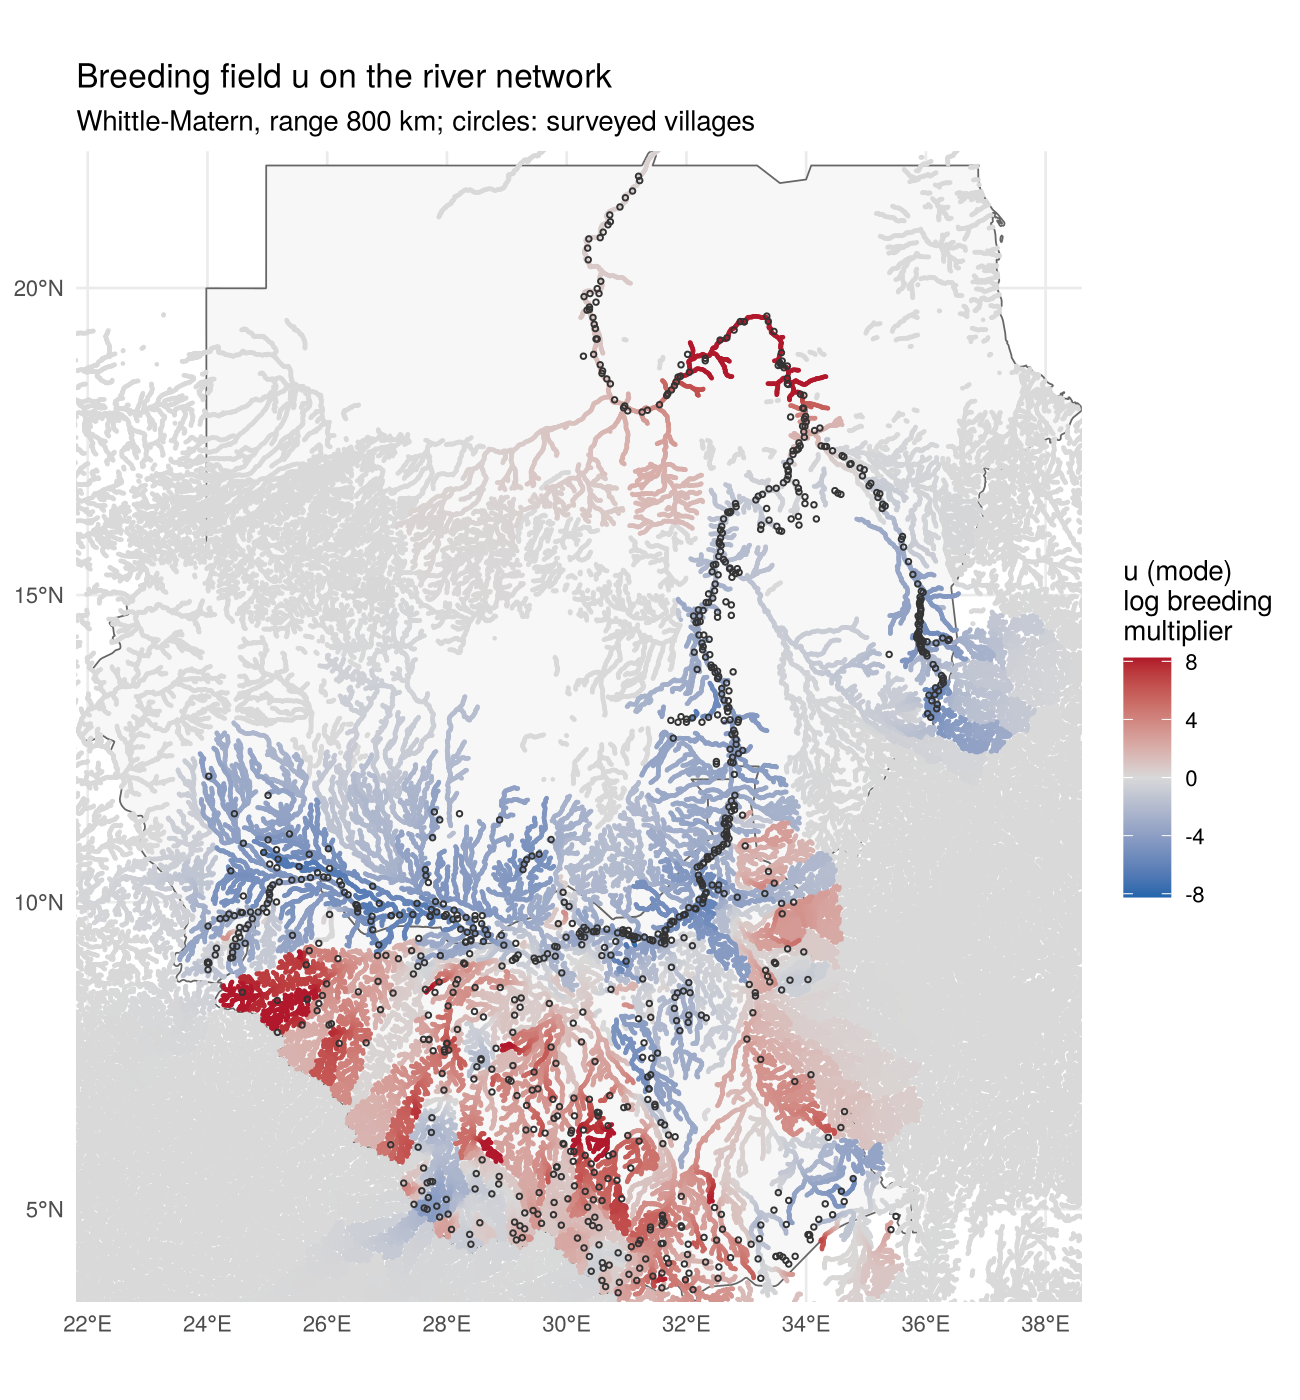
\includegraphics[width=0.49\textwidth]{zil_u_map.png}\hfill
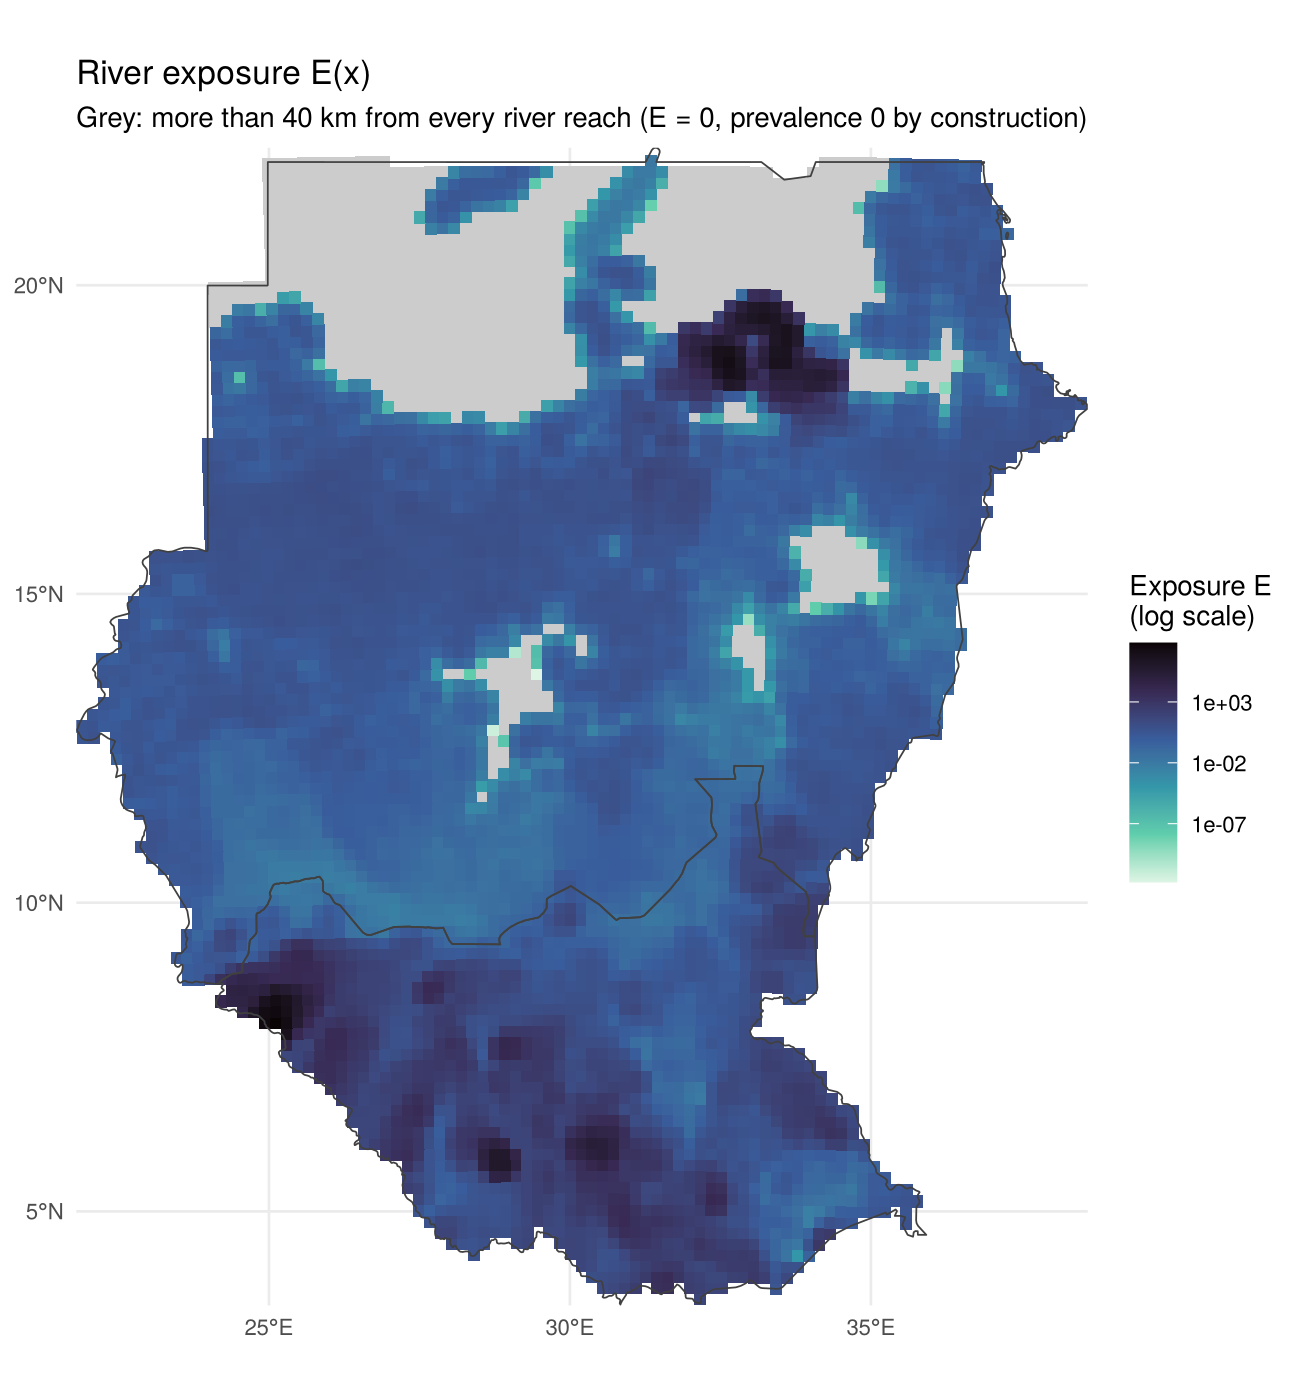
\includegraphics[width=0.49\textwidth]{zil_exposure_map.png}
\caption{Left: posterior mode of the breeding field $u$ (log multiplier of the breeding intensity) on the river network; circles are the surveyed villages. Right: river exposure $E(x)$ on a 20~km grid, on a logarithmic scale; grey cells lie more than 40~km from every reach, where $E = 0$.}
\label{fig:u}
\end{figure}

Figure~\ref{fig:Erivers} shows the exposure evaluated at points on the rivers themselves, about 4--8~km apart. Because a point on a river draws on the breeding along that river and on all other reaches within 40~km, this map combines the field $u$ with the density of the network and the effect of discharge. The exposure spans about seven orders of magnitude, from 0.01 to $2 \times 10^5$ between the 1st and 99th percentiles, with a median of 6. It is highest on the Nile between Abu Hamad and the Atbara confluence, on the dense networks of small streams in the far west and centre of South Sudan and in the south-east, and lowest along the Nile north of Abu Hamad, the White Nile, the Bahr el Ghazal and its tributaries, where the field $u$ is negative. On the unsurveyed seasonal streams of Darfur and Kordofan, where the data carry no information on $u$, the exposure is intermediate, of the order of 1--10, and reflects discharge and the density of the network alone; it is the low aridity index of these areas, through the probability of a zone, that keeps their predicted prevalence close to zero.

\begin{figure}[H]
\centering
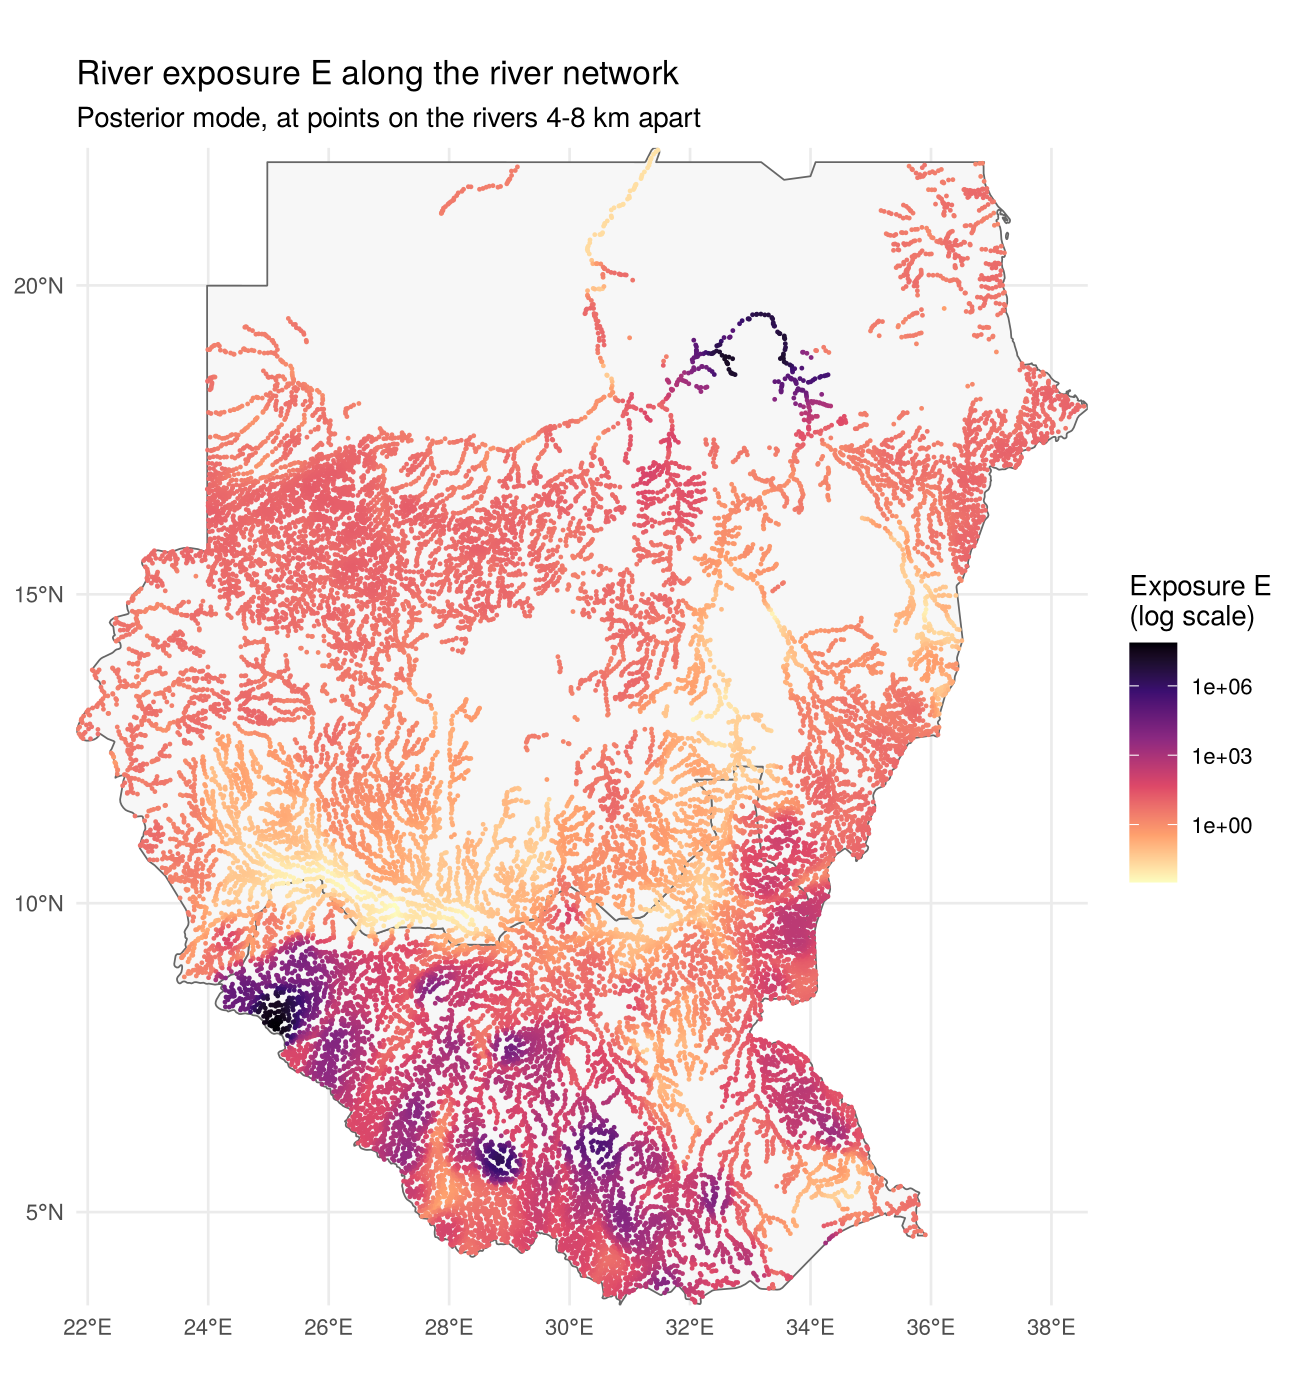
\includegraphics[width=0.75\textwidth]{zil_exposure_rivers.png}
\caption{River exposure $E$ evaluated at points on the river network, at the posterior mode of $u$ and $\theta$, on a logarithmic scale.}
\label{fig:Erivers}
\end{figure}

The probability that a surveyed village lies in a zone of transmission (Figure~\ref{fig:pi}, left) averages 0.06 for the hyper-arid villages, 0.01 for the arid, 0.33 for the semi-arid and 0.94 for the sub-humid and humid villages. It is close to zero along almost the whole of the Nile and the White Nile in Sudan and across the northern Sahel, high at the villages near Abu Hamad, intermediate along the White Nile through the Sudd swamps, whose slow water offers little breeding habitat, and close to one over most of South Sudan. On the prediction grid (Figure~\ref{fig:pi}, right) the same pattern holds away from the surveys: the probability of a zone is close to zero across the desert and the northern Sahel and rises sharply south of about 10\textdegree N.

\begin{figure}[H]
\centering
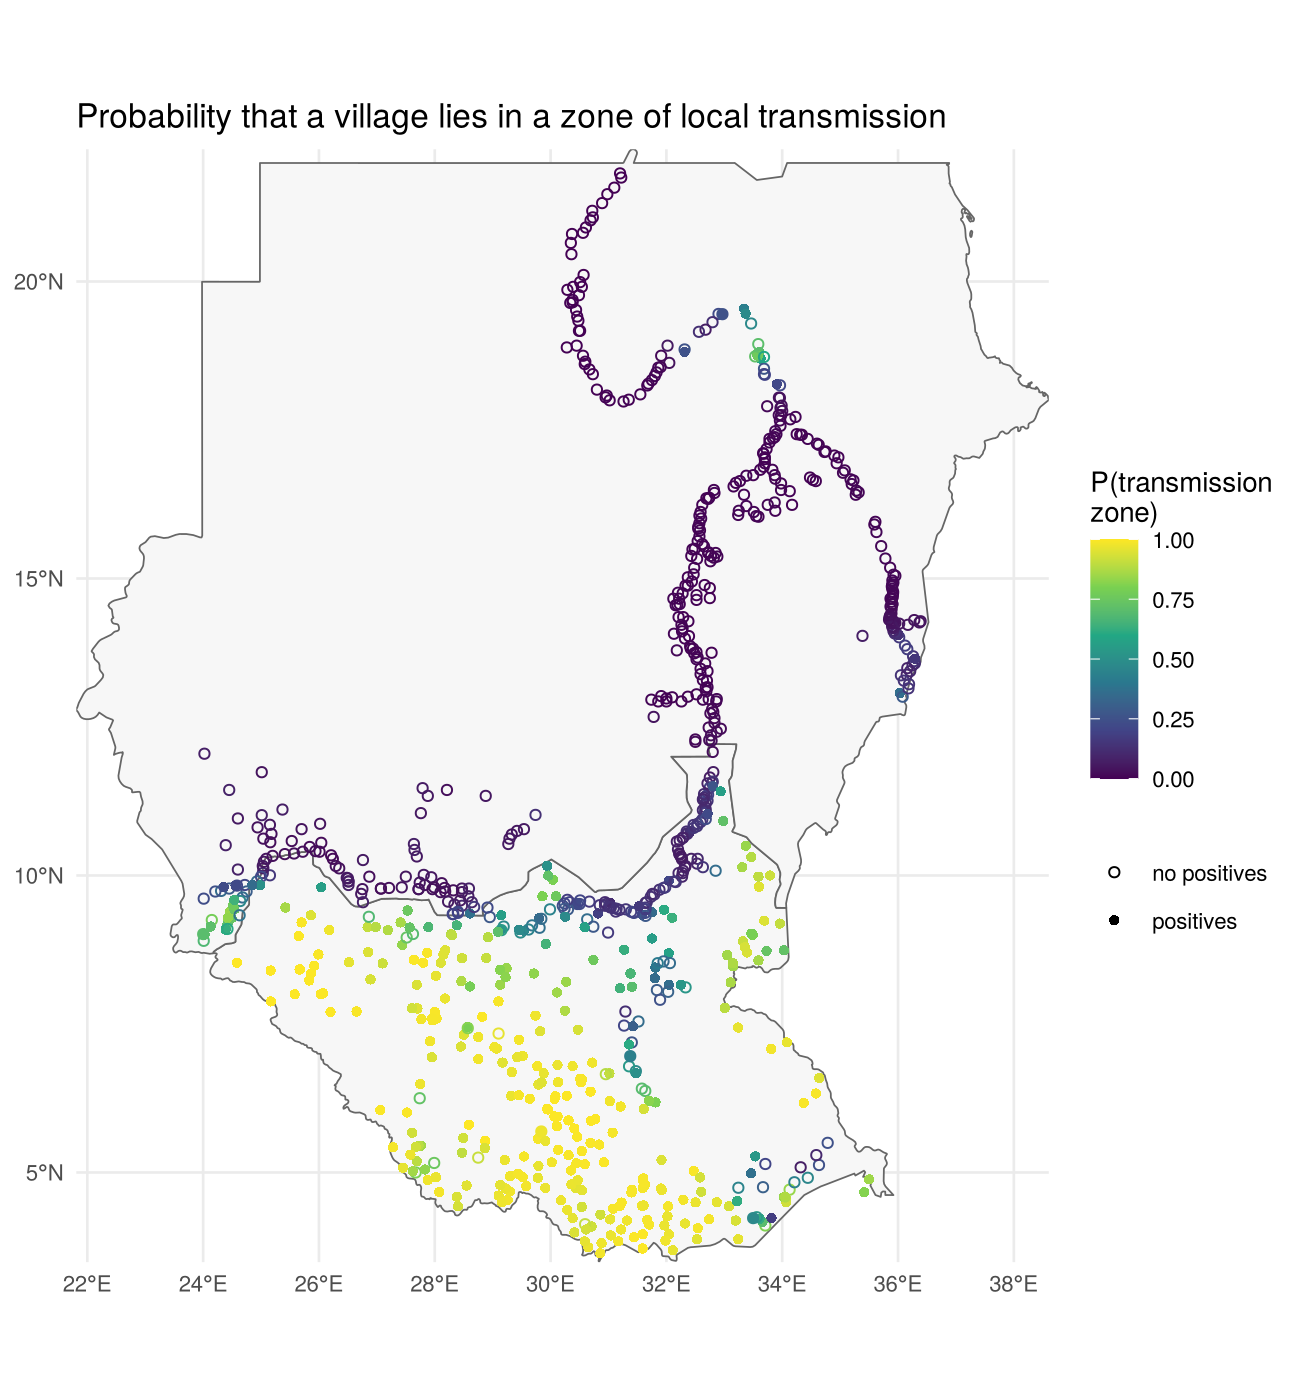
\includegraphics[width=0.49\textwidth]{zil_pi_villages.png}\hfill
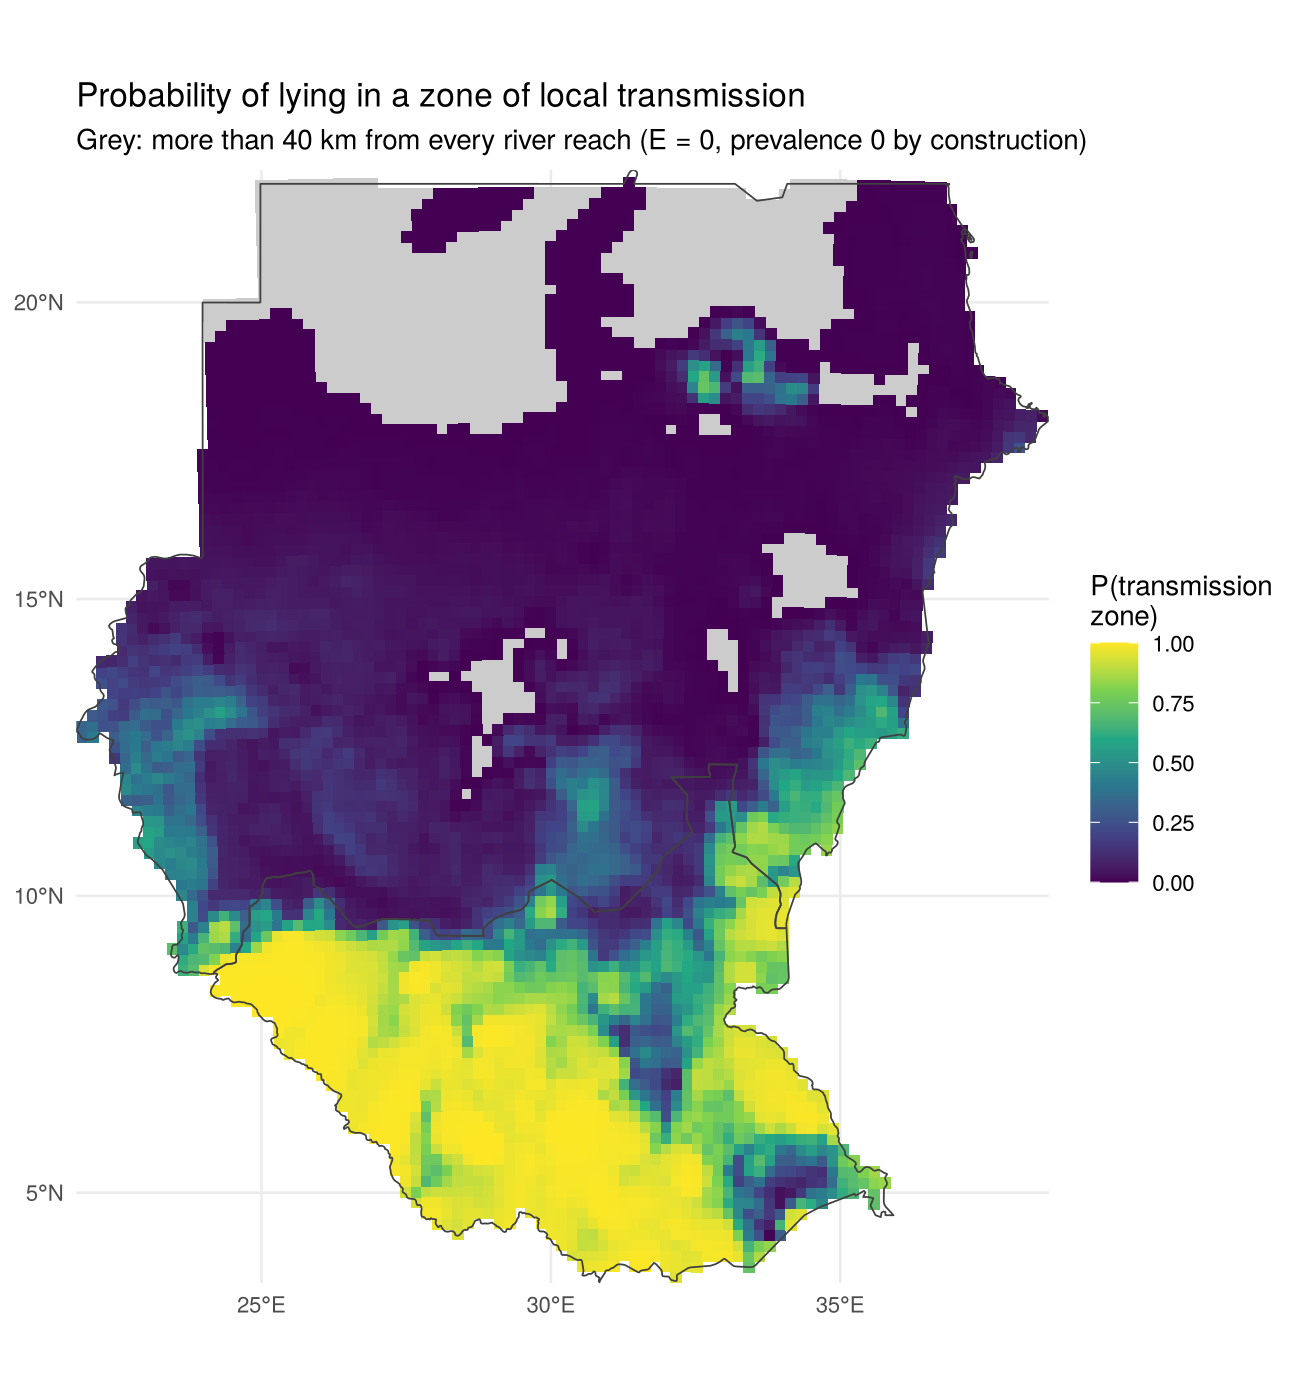
\includegraphics[width=0.49\textwidth]{zil_pi_map.png}
\caption{Probability of lying in a zone of local transmission, $\pi(x)$, at the posterior mode. Left: at the surveyed villages (filled symbols: villages with at least one positive). Right: on a 20~km grid; grey cells lie more than 40~km from every reach.}
\label{fig:pi}
\end{figure}

Within a zone, the prevalence $p(x)$ (Figure~\ref{fig:prev}, left) varies less: it is below 10\% over most of Sudan and between 20\% and 40\% over much of South Sudan, with the highest values in the far west of South Sudan, near the border with the Central African Republic, and in foci in the centre and south of South Sudan. The expected prevalence $\pi(x)p(x)$ (Figure~\ref{fig:prev}, right) is essentially zero across the desert and the Sahel, also far from the surveys: of the 3{,}691 arid and hyper-arid grid cells, three have an expected prevalence above 5\%. Infection is predicted mainly in South Sudan and along the southern margin of Sudan, with the highest values in the south-west.

\begin{figure}[H]
\centering
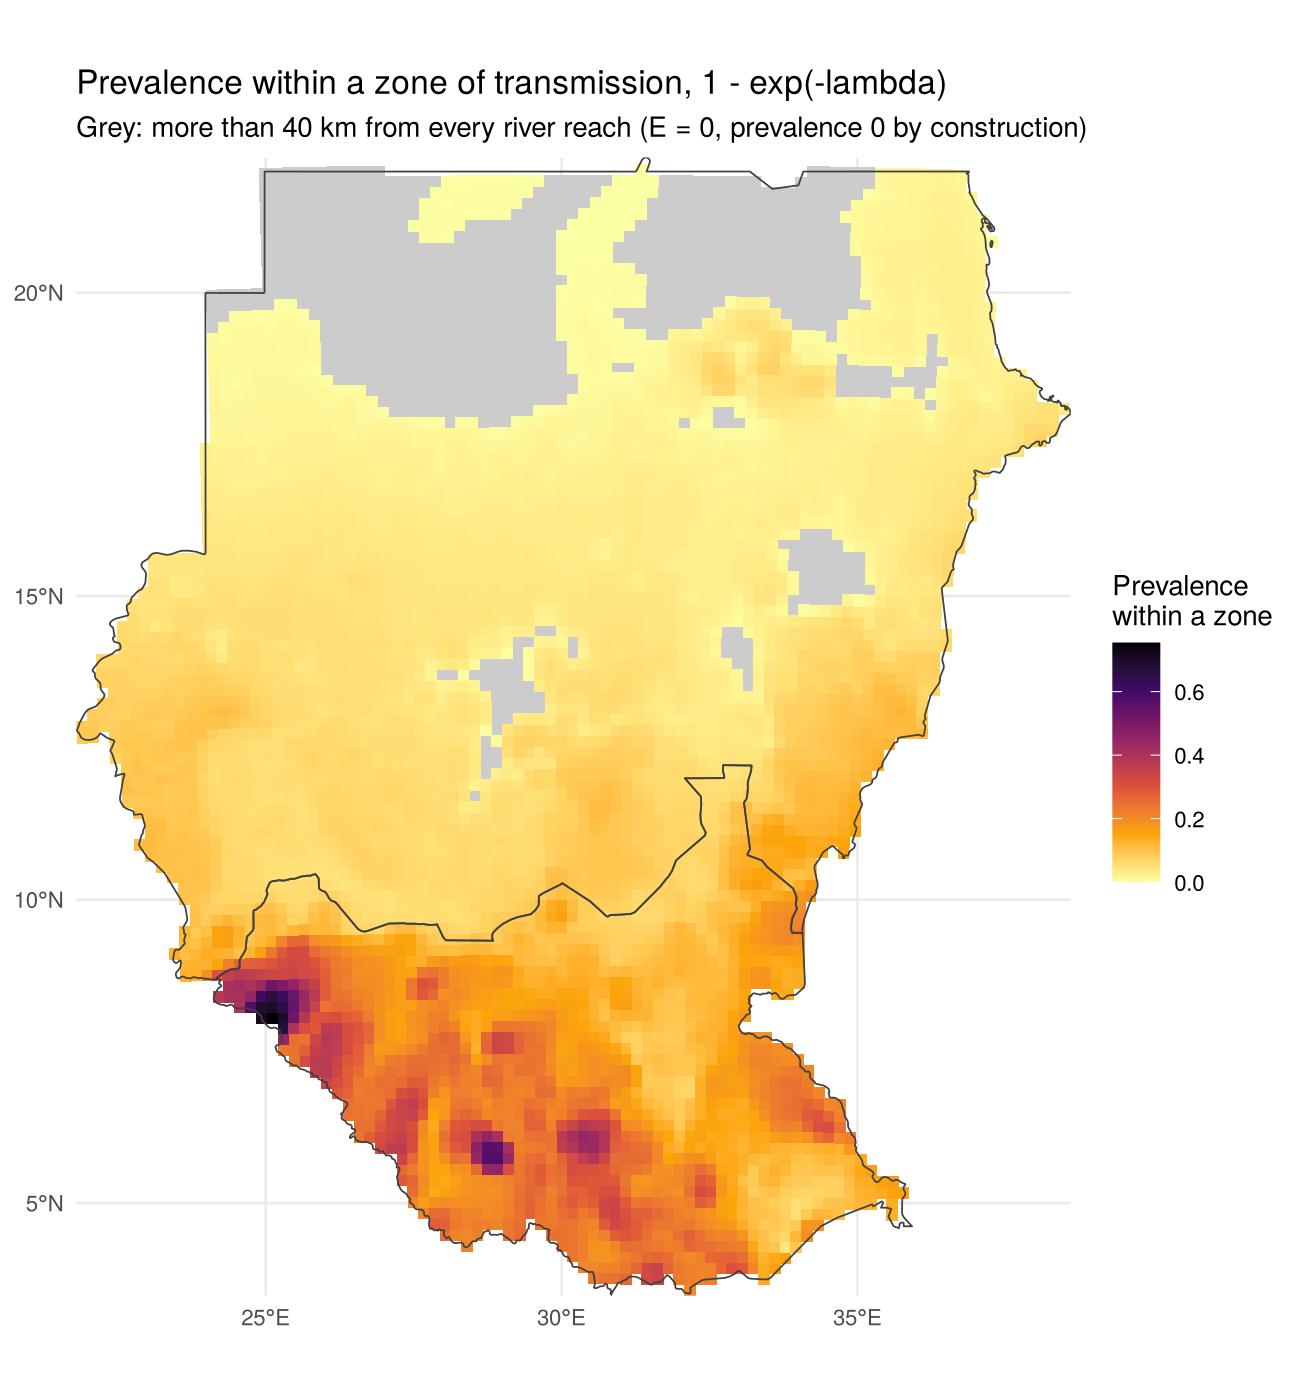
\includegraphics[width=0.49\textwidth]{zil_pzone_map.png}\hfill
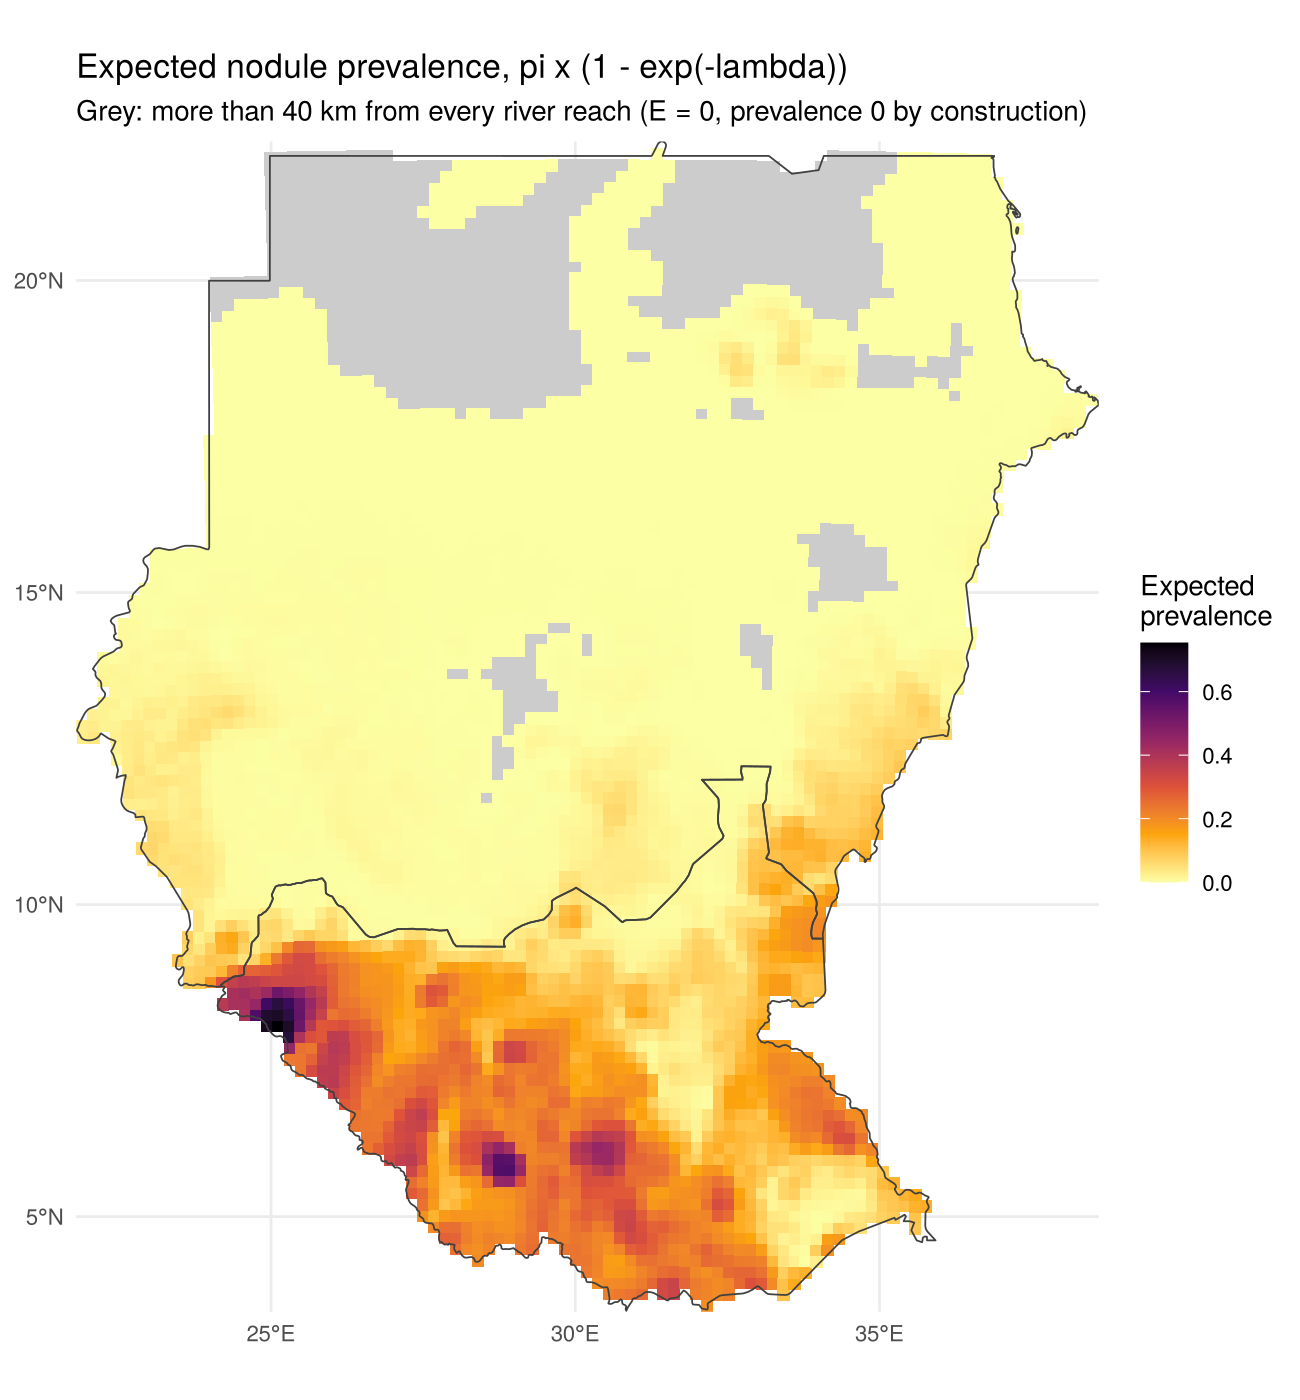
\includegraphics[width=0.49\textwidth]{zil_prevalence_map.png}
\caption{Left: prevalence within a zone of transmission, $p(x) = 1 - \exp\{-\lambda(x)\}$. Right: expected prevalence $\pi(x)p(x)$. Both on a 20~km grid, at the posterior mode with the village effect set to zero; grey cells lie more than 40~km from every reach.}
\label{fig:prev}
\end{figure}

Observed and predicted prevalence at the villages (Figure~\ref{fig:obs}) have a correlation of 0.87 in-sample and 0.76 under cross-validation, and the prevalence by aridity class is reproduced closely (Table~\ref{tab:classes}). The in-sample predictions use the mode of $u$ estimated from the same villages and so overstate predictive performance, whereas the cross-validated predictions are for villages not used in fitting. In both, the highest observed prevalences are underestimated, the more so under cross-validation, because a village effect, specific to each village, cannot be predicted for a new village, and because the predictive mean averages over the uncertainty in $u$; some villages without positives in the sub-humid zone have predicted prevalences of 20--35\%.

\begin{figure}[H]
\centering
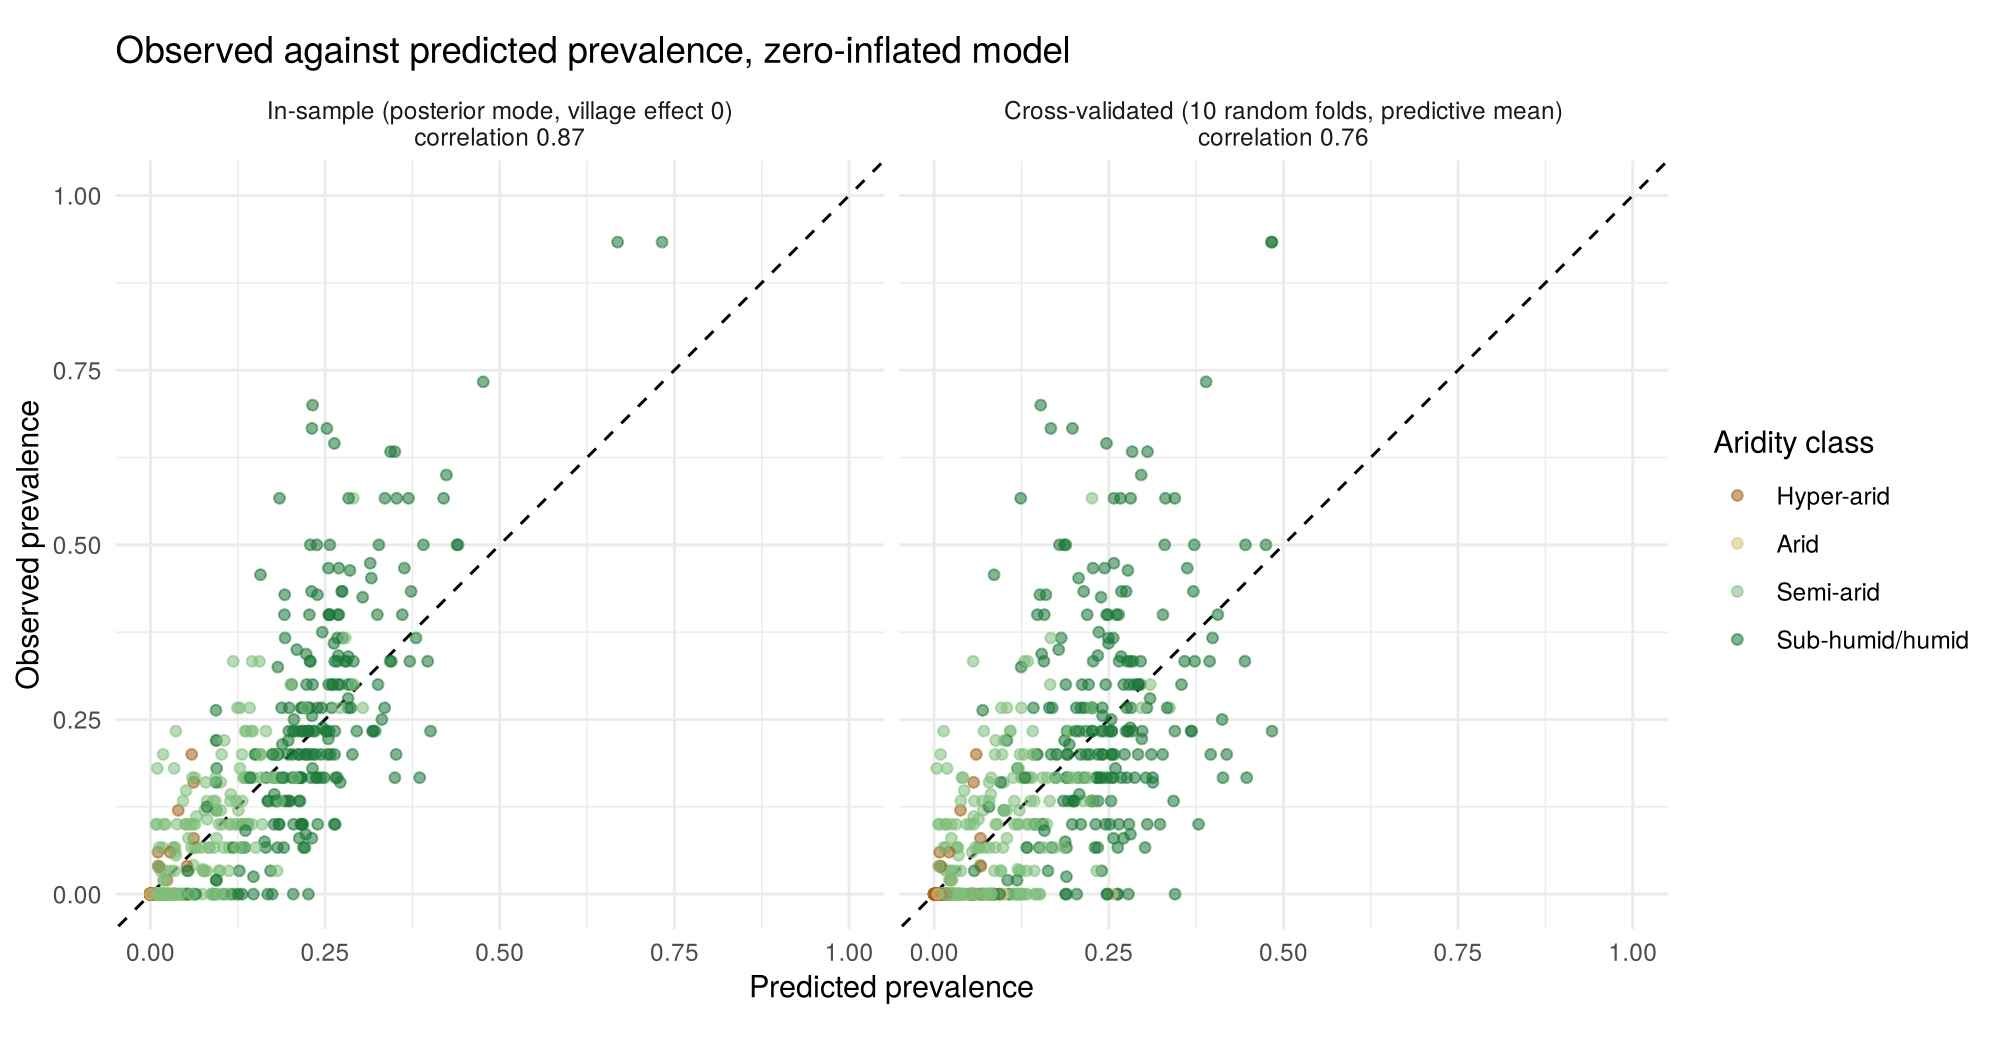
\includegraphics[width=\textwidth]{zil_obs_vs_pred.png}
\caption{Observed against predicted prevalence at the 900 villages. Left: in-sample, expected prevalence $\pi(x_i)p(x_i)$ at the posterior mode with the village effect set to zero. Right: ten-fold cross-validation with random folds, mean of the predictive distribution divided by the number examined.}
\label{fig:obs}
\end{figure}

\begin{table}[H]
\centering
\caption{Observed and in-sample predicted prevalence by aridity class (totals of positives over totals examined), and observed and cross-validated expected numbers of villages without positives.}
\label{tab:classes}
\begin{tabular}{lrrrrr}
\toprule
 & & \multicolumn{2}{c}{Prevalence} & \multicolumn{2}{c}{Villages without positives} \\
\cmidrule(lr){3-4}\cmidrule(lr){5-6}
Aridity class & Villages & Observed & Predicted & Observed & Expected (CV) \\
\midrule
Hyper-arid ($\AI < 0.05$) & 164 & 0.005 & 0.004 & 154 & 149.1 \\
Arid (0.05--0.20) & 107 & 0.000 & 0.000 & 107 & 99.3 \\
Semi-arid (0.20--0.50) & 404 & 0.033 & 0.035 & 275 & 270.1 \\
Sub-humid and humid ($\AI > 0.50$) & 225 & 0.252 & 0.234 & 14 & 25.2 \\
Total & 900 & & & 550 & 543.7 \\
\bottomrule
\end{tabular}
\end{table}

The cross-validated calibration is shown in Figure~\ref{fig:cv}. Among the 350 villages with at least one positive, the non-randomised PIT histogram is close to flat, with nine of its ten bins within the range expected under calibration; the one exception, a shortfall in the bin from 0.7 to 0.8, is not accompanied by a deficit or excess in the neighbouring bins, and the histogram shows neither the hump of over-dispersed nor the U-shape of under-dispersed predictive distributions. The predicted numbers of positives in villages where transmission occurs are therefore calibrated. The predicted probability of at least one positive separates villages with and without positives well, with an area under the ROC curve of 0.949, a Brier score of 0.084 and a mean logarithmic score of $-1.306$, and its reliability diagram lies close to the diagonal across the deciles of the prediction. The expected number of villages without positives, 543.7, is close to the 550 observed, also within each aridity class (Table~\ref{tab:classes}), with a modest excess of predicted zeros among the humid villages, 25 against 14 observed.

\begin{figure}[H]
\centering
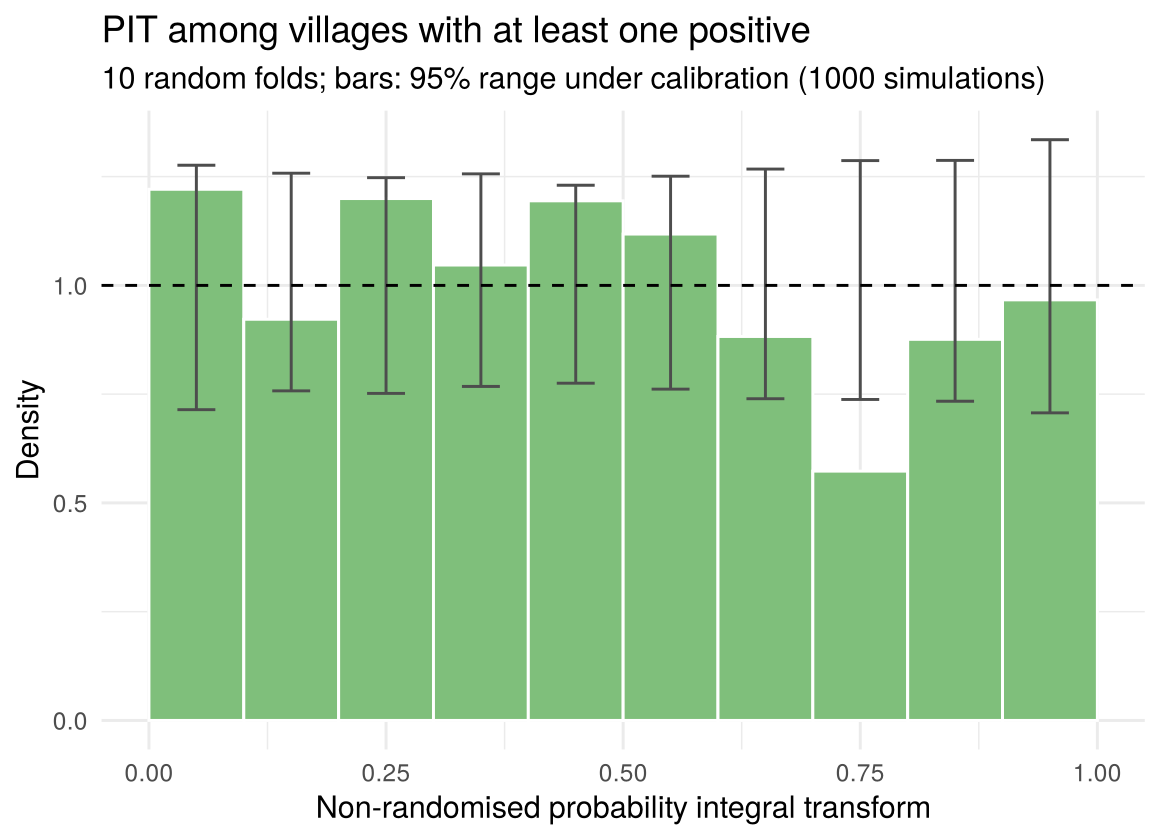
\includegraphics[width=0.56\textwidth]{zil_only_pit.png}\hfill
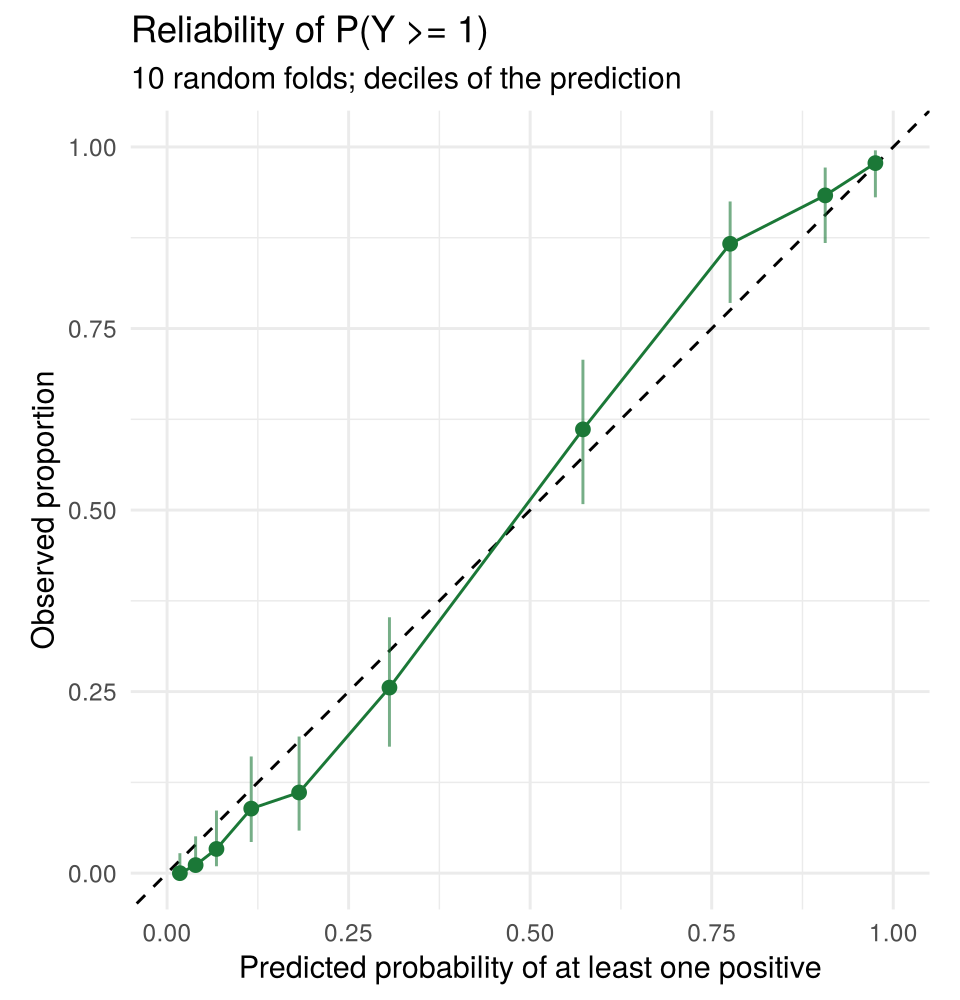
\includegraphics[width=0.42\textwidth]{zil_only_reliability.png}
\caption{Ten-fold cross-validation with random folds. Left: non-randomised PIT \citep{czado2009} among the 350 villages with at least one positive, conditional on $Y \geq 1$; bars show the 95\% range expected under calibration from 1{,}000 simulations. Right: reliability of the predicted probability of at least one positive, by deciles of the prediction, with 95\% intervals.}
\label{fig:cv}
\end{figure}

If the breeding field accounts for the spatial structure in the data, the village effects should be spatially independent. We assessed this with the empirical variogram of the predicted village effects, the posterior modes of $Z(x_i)$, in distance bins up to 300~km, with an envelope of spatial independence obtained by randomly permuting the predicted effects among the villages 9{,}999 times. The variogram is computed for the 350 villages with at least one positive. In this model the village effect acts only within a zone of transmission, so for a village without positives the data carry almost no information on it and its prediction is shrunk to about zero (variance of the predicted effects $4 \times 10^{-4}$, against 0.10 in villages with positives); because these villages are clustered, a variogram over all villages would be low at short distances through the shrinkage alone. Two tests are reported: a global test, based on the sum over bins of the squared standardised differences between the observed variogram and the mean of the permuted variograms, and a one-sided test of positive correlation, based on the sum of the standardised amounts by which the observed variogram falls below the permutation mean in the bins up to 100~km; in each the $p$-value is the rank of the observed statistic among the permuted ones.

The variogram (Figure~\ref{fig:variogram}) shows no positive spatial correlation in the village effects: at no distance does it fall below the permutation mean by more than chance, and the one-sided test gives $p = 1.00$. At distances up to 75~km it lies at or slightly above the upper limit of the envelope, and the global test, which is sensitive to departures in either direction, gives $p = 0.015$. A semivariance above the envelope means that neighbouring villages are less alike than random pairs, the opposite of positive correlation: neighbouring villages draw on the same stretches of river and share $u$, so their village effects are estimated as deviations around a common value. Because the predicted effects are shrunk by different amounts depending on the number examined and on the information about $u$, they are not exactly exchangeable, and the permutation test is a diagnostic rather than a formal test. We conclude that $u$ accounts for the spatial structure and that the village effect can be kept as independent.

\begin{figure}[H]
\centering
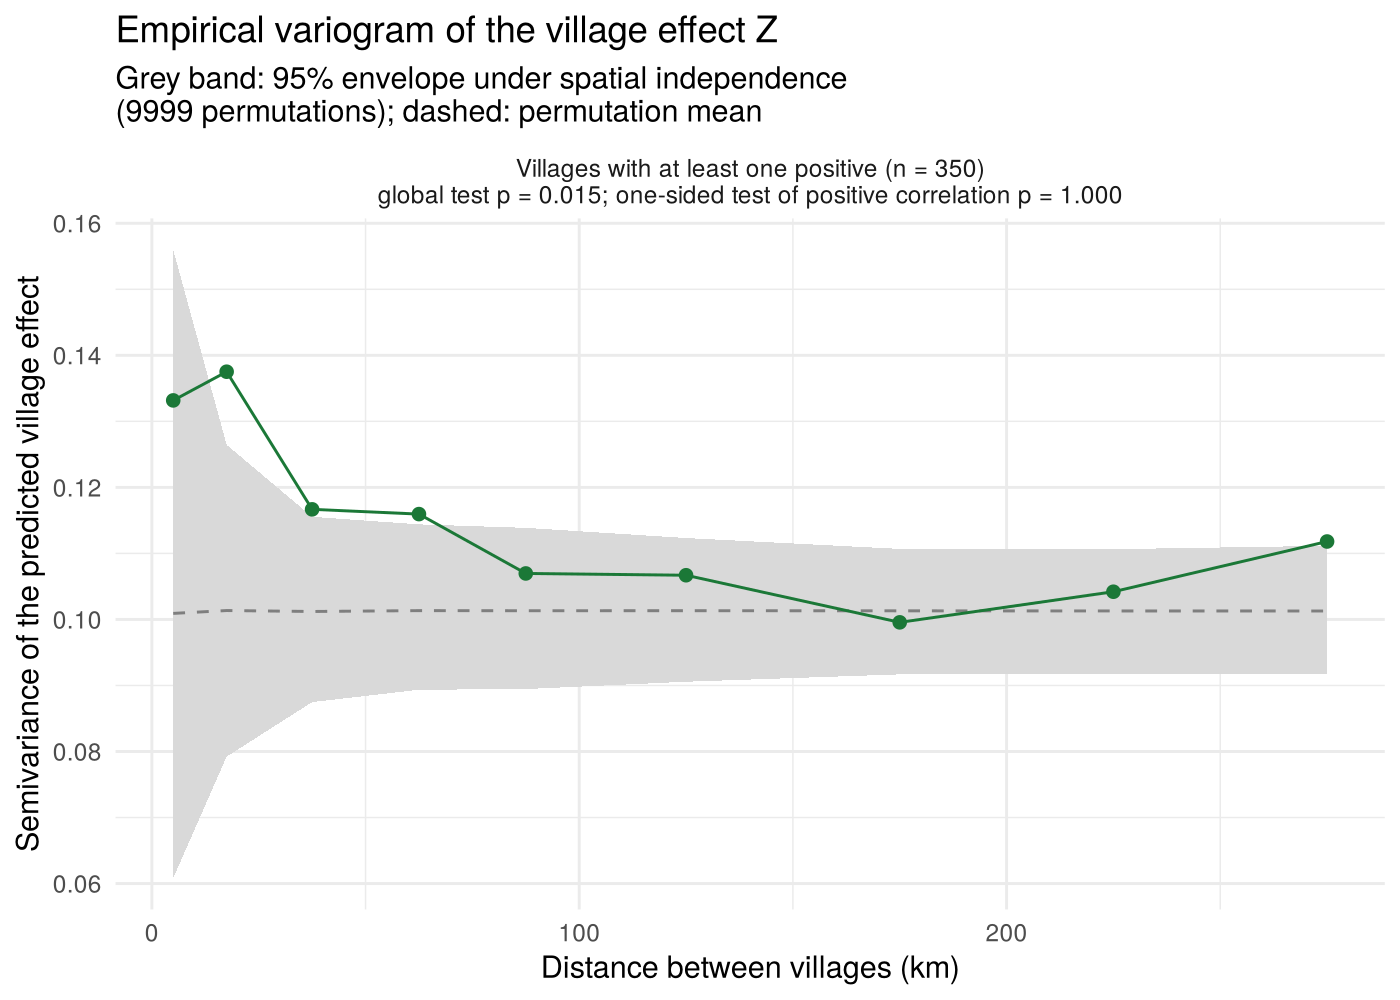
\includegraphics[width=0.72\textwidth]{variogram_z_zil.png}
\caption{Empirical variogram of the predicted village effect $Z$ among the 350 villages with at least one positive. Grey band: 95\% envelope under spatial independence from 9{,}999 random permutations of the predicted effects among the villages; dashed line: mean of the permuted variograms.}
\label{fig:variogram}
\end{figure}

\section{Discussion}

The model separates two questions that a binomial model with a village effect must answer together: whether a village lies in a zone where transmission occurs, and how intense transmission is when it does. Rivers and climate act mainly on the first, through the exposure from the network and the aridity index, and the separation is what makes the predictions calibrated, both for the number of villages without positives and for the numbers of positives where infection is found. Without zero inflation, the village effect had to be wide enough to produce the many villages without positives, which made the predictive distributions too wide for the villages with positives. The field $u$ maps the stretches of river that sustain transmission, among which the cataracts of the Nile near Abu Hamad stand out in the desert, and after it is included the village effects show no spatial correlation.

Several points need attention. The range of $u$ is fixed at the value estimated without zero inflation, and its variance is large; a profile over the range for this model, or a field with smoothness $\alpha = 2$, could be considered. Away from the rivers within reach of a surveyed village, $u$ returns to zero and its uncertainty is large, and predictions in unsurveyed basins inherit this uncertainty, which the plug-in maps at the posterior mode do not show; prediction uncertainty should be obtained by sampling from the Laplace approximation. Zero prevalence beyond 40~km of every river is imposed by the compact support of the dispersal kernel and the fixed dispersal range, not estimated; these areas are hyper-arid desert without survey data, where the model would in any case predict a very small probability of transmission. Finally, the field may be partly explained by measured river characteristics, such as channel gradient and the seasonality of flow, which would turn part of $u$ into interpretable covariates.

\begin{thebibliography}{9}

\bibitem[Bolin et al.(2024)]{bolin2024}
Bolin, D., Simas, A.~B. and Wallin, J. (2024).
\newblock Gaussian Whittle--Mat\'ern fields on metric graphs.
\newblock \textit{Bernoulli}, 30(2), 1611--1639.

\bibitem[Carnaghi et al.(2024)]{carnaghi2024}
Carnaghi, M. et al. (2024).
\newblock Short- and long-range dispersal by members of the \textit{Simulium damnosum} complex (Diptera: Simuliidae), vectors of onchocerciasis: a review.
\newblock \textit{Insects}, 15(8), 606.

\bibitem[Czado et al.(2009)]{czado2009}
Czado, C., Gneiting, T. and Held, L. (2009).
\newblock Predictive model assessment for count data.
\newblock \textit{Biometrics}, 65, 1254--1261.

\bibitem[Lehner and Grill(2013)]{lehner2013}
Lehner, B. and Grill, G. (2013).
\newblock Global river hydrography and network routing: baseline data and new approaches to study the world's large river systems.
\newblock \textit{Hydrological Processes}, 27, 2171--2186.

\bibitem[Steihaug(1983)]{steihaug1983}
Steihaug, T. (1983).
\newblock The conjugate gradient method and trust regions in large scale optimization.
\newblock \textit{SIAM Journal on Numerical Analysis}, 20(3), 626--637.

\bibitem[Wendland(1995)]{wendland1995}
Wendland, H. (1995).
\newblock Piecewise polynomial, positive definite and compactly supported radial functions of minimal degree.
\newblock \textit{Advances in Computational Mathematics}, 4, 389--396.

\bibitem[Zomer et al.(2022)]{zomer2022}
Zomer, R.~J., Xu, J. and Trabucco, A. (2022).
\newblock Version 3 of the Global Aridity Index and Potential Evapotranspiration Database.
\newblock \textit{Scientific Data}, 9, 409.

\end{thebibliography}

\end{document}
